\documentclass[../main/main.tex]{subfiles}

\newdate{date}{27}{11}{2019}


\begin{document}

Using the constraints
\marginpar{ \textbf{Lecture 13.} \\  \displaydate{date}. \\ Compiled:  \today.}
\begin{equation*}
  \begin{cases}
    \Tr^{(i)}(\rho _i) = 1  &\rightarrow  a+b=1\\
    \Tr^{(i)}(\rho _i S_i) = m_i  & \rightarrow b-a = m_i
  \end{cases}
\end{equation*}
where \( a,b \) are the functions of the order parameter.
In that case we have not to write the functions for all the \emph{i}. For \( S_i = 1 \) we have one value, for all the other values another one.
The results of the previous equation are:
\begin{equation*}
  \begin{cases}
   a = \frac{1-m_i}{2} \\
   b = \frac{1+m_i}{2}
  \end{cases}
\end{equation*}
Hence,
\begin{equation}
  \rho _i =   \frac{1-m_i}{2}  (1- \delta _{S_i,1}) + \frac{1+m_i}{2} \delta _{S_i,1}
\end{equation}
that in matrix form can be expressed as
\begin{equation}
\rho_i = 
\begin{pmatrix}
\frac{(m_i+1)}{2}   & 0 \\
  0 &    \frac{(1-m_i)}{2}
\end{pmatrix}
\end{equation}
\subsubsection{Mean field energy term}
Let us consider the average of the Hamiltonian
\begin{equation}
  \expval{\mathcal{H}}_{\rho _{MF}} = \expval{-J \sum_{\expval{ij} }^{} S_i S_j - \sum_{i}^{} H_i S_i   }_{\rho _{MF}}
  = - J   \sum_{\expval{ij} }^{} \expval{S_i S_j}_{\rho _{MF}} - \sum_{i}^{} H_i \expval{S_i}_{\rho _{MF}}
\end{equation}
Since we have
\begin{equation*}
  \rho _{MF} = \prod_{i=1}^{N} \rho _i
\end{equation*}
the term \( \expval{S_i S_j}_{\rho _{MF}}  \)  will transform into
\begin{equation*}
  \expval{S_i S_j}_{\rho _{MF}} = \expval{S_i}_{\rho _{MF}} \expval{S_j}_{\rho _{MF}}
\end{equation*}
Moreover, for all function \( g \) of \( S_i \) we can write
\begin{equation*}
\begin{split}
  \expval{g(S_i)}_{\rho _{MF}} &= \Tr^{(i)}(g(S_i)\rho _i) = \sum_{S_i = \pm 1}^{} g(S_i) \rho _i    \\
  &= \sum_{S_i = \pm 1}^{} g(S_i) \qty[\frac{1+m_i}{2} \delta _{S_i,1} + \frac{1-m_i}{2} (1- \delta _{S_i,1})  ] \\
  & = \frac{1+m_i}{2}g(1) + \frac{1-m_i}{2} g(-1)
\end{split}
\end{equation*}
Note that, if \( g(S_i) = S_i \), we have \( g(1) = +1\) and \( g(-1) = -1 \), hence
\begin{equation*}
  \expval{S_i}_{\rho _{MF}} = m_i
\end{equation*}
as expected. Taken this into account, the Hamiltonian can be rewritten as 
\begin{equation}
  \expval{\mathcal{H}}_{\rho _{MF}} = -J \sum_{\expval{ij} }^{} m_i m_j - \sum_{i}^{} H_i m_i
\end{equation}
\begin{remark}
This has the form of the original Hamiltonian where \( S_i \) had been replaced by their statistical averages.
\end{remark}
\noindent The entropy term is:
\begin{equation}
\begin{split}
  \expval{\ln{\rho } }_{\rho _{MF}} & = \Tr(\rho \ln{\rho } )  \overset{MF}{=} \sum_{i}^{} \Tr^{(i)} (\rho _i \ln{\rho _i} ) \\
 &  = \sum_{i}^{} \qty[ \frac{1+m_i}{2} \ln{\frac{1+m_i}{2}} + \frac{1-m_i}{2} \ln{\frac{1-m_i}{2}} ]
\end{split}
\end{equation}
The total free energy in Eq.\eqref{eq:12_3} becomes:
\begin{equation}
\begin{split}
  F_{\rho _{MF}} &= \expval{\mathcal{H}}_{\rho _{MF}} + k_B T \expval{\ln{\rho } }_{\rho _{MF}} \\
  & = - J \sum_{\expval{ij} }^{} m_i m_j - \sum_{i}^{} H_i m_i
  + k_B T   \sum_{i}^{} \qty[ \frac{1+m_i}{2} \ln{\frac{1+m_i}{2}} + \frac{1-m_i}{2} \ln{\frac{1-m_i}{2}} ]
\end{split}
\end{equation}
We now look for the values \( m_i = \bar{m_i}  \), that minimizes \( F_{\rho _{MF}} \) (equilibrium phases):
\begin{equation*}
 \eval{ \pdv{F_{\rho _{MF}} }{m_i} }_{m_i = \bar{m_i} } = 0
\end{equation*}
This gives:
\begin{equation*}
  0 = - J \sum_{j \in \, n.n. \,\text{of}\, i}^{} \bar{m_j} - H_i + \frac{k_B T}{2} \ln{\qty[\frac{1+\bar{m_i} }{1- \bar{m_i} }] }
\end{equation*}

To solve it, remember that
\begin{equation*}
  \tanh^{-1} (x) = \frac{1}{2} \ln{\frac{1+x}{1-x}} \quad |x| < 1
\end{equation*}
Hence,
\begin{equation*}
  k_B T \tanh^{-1} ( \bar{m_i} ) = J \sum_{j \in \, n.n. \,\text{of}\, i}^{} \bar{m_j} + H_i
\end{equation*}
which implies
\begin{equation*}
  \bar{m_i} = \tanh \qty[(k_B T)^{-1} \qty(J \sum_{j \in \, n.n. \,\text{of}\, i}^{} \bar{m_j} + H_i ) ]
\end{equation*}
We have again found the self-consistency equation for the magnetization that we have already encountered in the Weiss mean field theory for the Ising model! This is again a confirmation that all mean field theories are equivalent.
Defining
\begin{equation*}
  z \bar{m_i} \equiv  \sum_{j \in \, n.n. \,\text{of}\, i}^{} \bar{m_j}
\end{equation*}
we get
\begin{equation}
  \bar{m_i} = \tanh \qty[\beta \qty(Jz \bar{m_i} +H_i) ]
\end{equation}
this is the Bragg-William approximation.


\begin{figure}[h!]
\begin{minipage}[c]{0.5\linewidth}
\subfloat[][Square lattice is bipartite.]{ 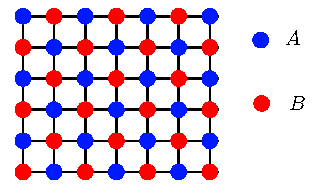
\includegraphics[width=0.8\textwidth]{../lessons/13_image/1.pdf}  \label{fig:} }
\end{minipage}
\begin{minipage}[]{0.5\linewidth}
\centering
\subfloat[][Triangular lattice is not bipartite.]{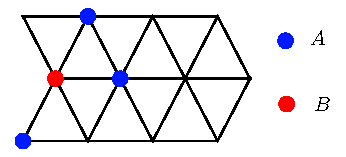
\includegraphics[width=0.8\textwidth]{../lessons/13_image/2.pdf}  \label{fig:} }
\end{minipage}
\caption{\label{fig:13_1} Ising anti-ferromagnet in an external field.}
\end{figure}


\begin{example}{Ising anti-ferromagnet in an external field}{}
Let us consider the model

\begin{equation}
  \mathcal{H} = \mathcolorbox{green!20}{+} J \sum_{\expval{ij} }^{} S_i S_j - H \sum_{i}^{} S_i,
\end{equation}
Note the \( + \) sign before \( J \), this means that the interactions are anti-ferromagnetic. Let us consider two cases:
\begin{itemize}
\item  If \( H=0 \) ferromagnetic and anti-ferromagnetic behave similarly when the interactions are between nearest neighbours on a \emph{bipartite lattice}, i.e. a lattice that can be divided into two sublattices, say \( A \) and \( B \), such that a \( A \) site has only \( B \) neighbours and a \( B \) site only \( A \) ones.
\begin{remark}
FCC is not bipartite, while BCC it is. See Figure \ref{fig:13_1}.
\end{remark}

If the lattice is bipartite and \( J_{ij} \) is non zero only when \( i \) and \( j \) belong to different sublattices (they do not have to be only n.n.!), one can redefine the spins such that
\begin{equation*}
  S_j' = \begin{cases}
    + S_j & j \in A \\
    - S_j & j \in B
\end{cases}
\end{equation*}
Clearly, \( S_i'S_j' = - S_i S_j \). It is like if the \( J_{ij} \) have changed sign and we are formally back to ferromagnetic model for the two sublattices:
\begin{equation}
  \mathcal{H}^{*} = \mathcolorbox{green!20}{-} J \sum_{\expval{ij} }^{} S_i' S_j'
\end{equation}
i.e. a ferromagnetic Ising.

\item In presence of a magnetic field \( H \), we need to reverse its sign when applied to sites \( B \).

The thermodynamic of a ferromagnetic Ising model on a bipartite lattice in a uniform magnetic field \( H \) is identical to the one of the Ising antiferromagnetic model in presence of the so called \emph{staggered field}, i.e. \( H_A = H \) and \( H_B = -H \).
The Hamiltonian is 
\begin{equation}
  \mathcal{H}^* [S] = -J \sum_{\expval{r_A r_B} }^{} S(r_A) S(r_B) - H \sum_{r_A}^{} S(r_A) + H \sum_{r_B}^{} S(r_B), \quad J>0, H>0
\end{equation}
The average magnetization per spin is
\begin{equation*}
  m \equiv \frac{1}{2}(m_A+m_B)
\end{equation*}
  while
  \begin{equation*}
    m_S = \frac{1}{2}(m_A-m_B)
  \end{equation*}
  is the \emph{staggered magnetization}.

In order to use the variational density matrix method for this problem we consider two independent variational parameters \( m_A \) and \( m_B \) for sublattice \( A \) and \( B \) respectively. On each sublattice, the model is like the standard Ising
\begin{equation*}
  \begin{cases}
   \rho _A^{(1)}(S) = \frac{1+m_A}{2} \delta _{S,1}+ \frac{1-m_A}{2}\delta _{S,-1}\\
   \rho _B^{(1)}(S) = \frac{1+m_B}{2} \delta _{S,1}+ \frac{1-m_B}{2}\delta _{S,-1}
  \end{cases}
\end{equation*}
\begin{remark}
Note that, being \( H \) uniform, \( \expval{S_i} = m \), i.e. does not depend on \( i \). Same for the \( 1- \)particle distribution functions \( \rho _A^{(1)}(S) \) and  \( \rho _B^{(1)}(S) \).
\end{remark}
By performing the calculation for the terms
\begin{equation*}
  \expval{\mathcal{H}}_{\rho _{MF}} = - J \sum_{\expval{ij} }^{} \expval{S_i S_j}_{\rho _{MF}} - H \sum_{i}^{} \expval{S_i}_{\rho _{MF}}
\end{equation*}
\begin{equation*}
  \expval{\ln{\rho } }_{\rho _{MF}} = \sum_{i}^{} \Tr^{(i)}(\rho _i \ln{\rho _i} )
\end{equation*}
as before, but remembering to partition the procedure into the two sublattices \( A \) and \( B \), one can show that the variational free energy is given by
\begin{equation}
  \frac{F(m_A,m_B)}{N} = \frac{z \hat{J} }{2}m_A m_B - \frac{1}{2}H (m_A+m_B)
  - \frac{1}{2} k_B T s(m_A) - \frac{1}{2}k_B T s(m_B)
\end{equation}
where the entropy term is 
\begin{equation*}
  s(m) = \qty[\frac{1+m}{2} \ln{\qty(\frac{1+m}{2}) } + \frac{1-m}{2} \ln{\qty(\frac{1-m}{2}) }  ]
\end{equation*}
By differentiating \( \frac{F}{N} \) with respect to \( m_A \) and \( m_B \), one gets
\begin{subequations}
\begin{align*}
   \pdv{(F/N)}{m_A} &= 0 & \Rightarrow m_B = \frac{H}{z \hat{J} } - \frac{k_B T}{z \hat{J} }\ln{\qty(\frac{1+m_A}{1-m_A}) } \\
   \pdv{(F/N)}{m_B} &= 0 & \Rightarrow m_A = \frac{H}{z \hat{J} } - \frac{k_B T}{z \hat{J} }\ln{\qty(\frac{1+m_B}{1-m_B}) }
\end{align*}
\end{subequations}
As before, since
\begin{equation*}
  \tanh^{-1} (x) = \frac{1}{2} \ln{\frac{1+x}{1-x}}
\end{equation*}
these self-consistent equations can be written as
\begin{equation}
  \begin{cases}
   m_A = \tanh ( \beta \qty(H - z \hat{J} m_B ) )\\
   m_B = \tanh ( \beta \qty(H - z \hat{J} m_A ) )
  \end{cases}
\end{equation}
The sites \( \in A \) experience an internal field \( H_{A,MF} = - z \hat{J} m_B \) from the \( B \) neighbours and vice versa for the sites \( \in B \).
\end{itemize}
\end{example}

\subsection{Second approach: Blume-Emery-Griffith model}
We apply this approach to the so called \emph{Blume-Emery-Griffith model}.
This is a spin model with vacancies that describes the phase diagram and the critical properties of an interacting system displaying a \emph{tricritical point}. Perhaps the most famous of these systems is the \( \text{He}^3-\text{He}^4 \) mixture undergoing a fluid-superfluid transition.

\begin{remark}
\( \text{He}^4 \)  is a non radiative isotope with two protons and two neutrons. Roughly \( 1/4 \) of the universe matter is \( \text{He}^4 \)!
From a quantum statistical point of view \( \text{He}^4 \) is a \emph{boson}.
\end{remark}

 A gas of \( \text{He}^4 \) undergoes a fluid-superfluid transition at \( T_ \lambda =2.17 K \) and \( P=P_0 \). It is known as \( \lambda - \)transition since at \( T \sim T_ \lambda  \)  the specific heat \( c(T) \) behaves as in Figure \ref{fig:13_2_1}: the plot of the specific heat as a function of the temperature has a shape that resembles a \(\lambda\). 
The \( \lambda - \)transition is a genuine critical point (second order). For \( T < T_{\lambda } \), \( \text{He}^4 \)  is in the superfluid phase and it can be described by a two-fluids model in which one component has zero viscosity and zero entropy.


\begin{figure}[h!]
\begin{minipage}[c]{0.5\linewidth}
\subfloat[][Plot of the specific heat \(c(T)\). It has the shape of a \(\lambda\).]{ 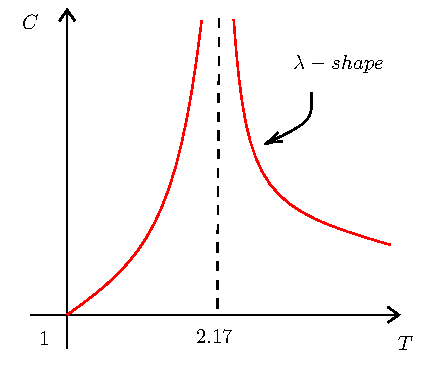
\includegraphics[width=0.9\textwidth]{../lessons/13_image/3.pdf}  \label{fig:13_2_1} }
\end{minipage}
\begin{minipage}[]{0.5\linewidth}
\centering
\subfloat[][\( (P,T) \) phase diagram.]{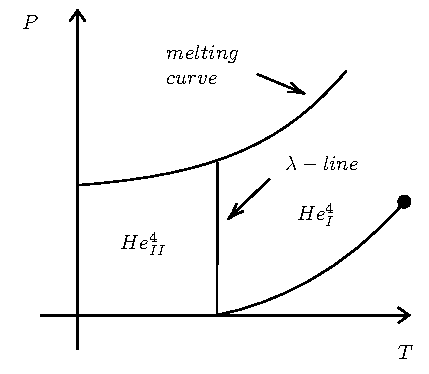
\includegraphics[width=0.9\textwidth]{../lessons/13_image/4.pdf}  \label{fig:13_2_2} }
\end{minipage}
\caption{\label{fig:13_2} }
\end{figure}

 The BEG model is used to describe what happens when we add some \( \text{He}^3 \) to the system constituted by \( \text{He}^4 \); it does not consider quantum effects, but only the "messing up" due to the \( \text{He}^3 \) impurities.
 
 \begin{remark}
  
\( \text{He}^3 \) is a non-radioactive isotope with 2 protons and 1 neutron. From a quantum statistical point of view is a \emph{fermion}.
 \end{remark}

Experimentally when \( \text{He}^3 \)
 is added to \( \text{He}^4 \) the temperature of the fluid-superfluid transition decreases. 
More specifically, if inserted in a system of \( \text{He}^4 \) it will "dilute" its bosonic property. Then, one expects that \( T_ \lambda  \) decreases, as observed. Denoting by \( x \) the concentration of \( \text{He}^3 \),  one observes
\begin{equation*}
  T_{\lambda} = T_ \lambda (x)
\end{equation*}
with \( T_ \lambda (x) \)  that decreases as \( x \) increases.

For small concentration of \( \text{He}^3 \) the mixture remains homogeneous, and the only effect is the change of \( T_ \lambda  \). However, when the concentration \(x\) of \( \text{He}^3 \) reaches the critical value \(x_t\)
\begin{equation*}
  x > x_t = \frac{n_3}{n_3+n_4} \sim 0.67
\end{equation*}
\( \text{He}^3 \) and \( \text{He}^4 \) separate into two phases  (just like oil separates from water, the mixture undergoes a separation between a phase rich and a phase poor of \( \text{He}^3 \))  and the \(\lambda\) transition becomes first-order (namely, discontinuous). The transition point \( (x_t,T_t) \) where the system shifts from a continuous \(\lambda\)-transition to a discontinuous one is that where the phase separation starts and is called tricritical point (i.e. it is a critical point that separates a line of second order transition from a line of first order transition). 
The BEG model was introduced to describe such a situation.


\subsubsection{BEG Model}
As we have anticipated, the BEG Model is a lattice gas model and so it is based on an Ising-like Hamiltonian. In particular, it is the model of a diluted ferromagnetic system.
On the sites of this lattice we define a variable \(S_i\) which can assume the values \(-1\),\(0\) and \(+1\): we decide that when an \( \text{He}^4 \) atom is present in a lattice site then  \(S_{i}=\pm 1\), while when \(S_{i}= 0\) it means that the site is occupied by an \( \text{He}^3 \) atom.
We then define our order parameter to be
\begin{equation*}
     \expval{S_i} = m_i 
\end{equation*}
In the Ising model  \( \expval{S_i^2}  \) can only be equal to \(1\), while in this case it can be either \(0\) or \(1\): we can thus interpret \( \expval{S_i^2}  \) as the concentration of \( \text{He}^4 \) atoms, and
\begin{equation*}
  x \equiv 1 - \expval{S_i^2}
\end{equation*}
 as the fraction of \( \text{He}^3 \).
 We also define 
\begin{equation*}
  \Delta \propto \mu _{\text{He}^3} - \mu _{\text{He}^4}
\end{equation*}
to be the difference of the chemical potentials of \( \text{He}^3 \) and \( \text{He}^4 \); since this parameter is related to the number of \( \text{He}^3 \) and \( \text{He}^4 \) atoms, we expect that when
\begin{itemize}
\item \( x \rightarrow 0\)  (namely, there is only \( \text{He}^4 \)), we have \( \Delta \rightarrow - \infty  \).
\item \( x \rightarrow 1\)  (namely, there is only \( \text{He}^3 \)), we have \( \Delta \rightarrow + \infty  \).
\end{itemize}
and the order parameter for the \( \lambda - \)transition becomes
\begin{equation*}
\expval{S_i} =
  \begin{cases}
   0 & T > T_{\lambda }\\
   m & T < T_{\lambda }
  \end{cases}
\end{equation*}
We consider the following Hamiltonian for the system:
\begin{equation}
\mathcal{H} = - J \sum_{\expval{ij} }^{N} S_i S_j + \Delta \sum_{i=1}^{N} S_i^2 - \Delta N
\end{equation}
\begin{remark}
\(N\) is the total number of lattice sites
The \( \Delta N \) term is a typical term for a gas in gran canonical ensemble.  
\end{remark}


\subsubsection{Variational mean field approach to BEG}
Since we want to apply the second variational method that we have seen, we write the mean field probability density as:
\begin{equation*}
  \rho _{MF} = \prod_{i}^{} \rho _i   =  \prod_{i}^{} \rho^{(1)} (S_i)
\end{equation*}
and the free energy:
\begin{equation}
  G(T,J,\Delta ) = \expval{\mathcal{H}}_{\rho _{MF}} + k_B T \sum_{i}^{} \Tr^{(i)}(\rho _i \ln{\rho _i } )
\end{equation}
The mean value of the Hamiltonian is:
\begin{equation*}
\expval{\mathcal{H}}_{\rho _{MF}}   = - J \sum_{\expval{ij} }^{} \expval{S_i S_j}  + \Delta \sum_{i}^{} \expval{S_i^2} - N \Delta  
\end{equation*}
and since \(\expval{S_i S_j} = \expval{S_i} \expval{S_j} \) (it's the fundamental hypothesis of mean field theories) we get
\begin{equation*}
\expval{\mathcal{H}}_{\rho _{MF}} \overset{MF}{\simeq } - J \sum_{\expval{ij} }^{} \expval{S_i} \expval{S_j} + \Delta \sum_{i}^{} \expval{S_i^2} - N \Delta   
\end{equation*}
We have also
\begin{equation*}
  \expval{S_i} = \expval{S_j} \equiv m
\end{equation*}
Therefore, the free energy of the system is:
\begin{equation}
  G(T,J, \Delta )_{MF}  = - \frac{1}{2} N J z \qty( \Tr_{S_i}(\rho _i S_i) )^2
  + N \Delta \Tr_{S_i}(\rho _i S_i^2) - N \Delta +
  N k_B T \Tr_{S_i}(\rho _i \ln{\rho _i} )
\end{equation}
where \(z\) is the coordination number of the lattice.

We now must minimize this expression with respect to \( \rho _i \), with the constraint 
\( \Tr_{S_i}(\rho _i) = 1  \):
\begin{equation*}
  \dv{G}{\rho _i} = 0
\end{equation*}
Let us consider each term
\begin{subequations}
\begin{align*}
  \dv{}{\rho_i} \qty(\Tr(\rho _i S_i) )^2& = 2 \qty(\Tr(\rho _i S_i) ) S_i = 2 \expval{S_i} S_i = 2 m S_i \\
    \dv{}{\rho_i} \qty(\Tr(\rho _i S_i^2) ) &= S_i^2 \\
      \dv{}{\rho_i} \qty(\Tr(\rho _i \ln{\rho _i} ) ) &=  \ln{\rho _i }  +1
\end{align*}
\end{subequations}
then,
\begin{equation*}
  \dv{G}{\rho _i}  = - J N z m S_i + N \Delta  S_i^2 + N k_B T \ln{\rho _i} + N k_B T = 0
\end{equation*}
Dividing by \( N k_B T \),
\begin{equation*}
  \ln{\rho _i} \equiv \ln{\rho ^{(1)} (S_i)} =   \beta J z m S_i - \beta \Delta S_i^2 - 1
\end{equation*}
which leads to
\begin{empheq}[box=\myyellowbox]{equation}
  \rho ^{(1)} (S_i) = \frac{1}{A} e^{\beta (zJmS_i - \Delta S_i^2)}
\end{empheq}
where we have reabsorbed \( e^{-1}  \) into the normalization constant \(A\).
The constant \( A \) can be found by imposing the constraint \( \Tr_{S_i}\rho ^{(1)}(S_i) =1 \), we find
\begin{empheq}[box=\myyellowbox]{equation}
  A = 1 + 2 e^{-\beta \Delta } \cosh (\beta z J m)
\end{empheq}
\begin{example}{How to compute \(A\)}{}
By imposing the constraint \( \Tr_{S_i}\rho ^{(1)}(S_i) =1 \) (recall that \(S_i=\pm1,0\)), we get 
\begin{equation*}
 1 = \frac{1}{A} \qty( e^{\beta (zJm(+1) - \Delta (+1)^2)}  + e^{\beta (zJm(-1) - \Delta (-1)^2)} + e^{\beta (zJm(0) - \Delta (0)^2)} )  
\end{equation*}
Hence, by rearranging 
\begin{equation*}
 1 = \frac{1}{A}  \qty( 2 e^{-\beta \Delta} \cosh{(\beta z J m)} + 1) \Rightarrow
  A = 1 + 2 e^{-\beta \Delta } \cosh (\beta z J m)
\end{equation*}
\end{example}

Given \( \rho ^{(1)}(S_i) \) it is possible to show 
\begin{equation*}
  \expval{S_i^2} = \Tr_{S_i}(\rho _i S_i^2) = \frac{1}{A} 2 e^{-\beta \Delta } \cosh ( \beta z J m)
\end{equation*}
and
\begin{equation*}
  x = 1 - \expval{S_i^2} = \frac{A - 2 e^{-\beta \Delta } \cosh (\beta z J m) }{A} \quad \Rightarrow x = \frac{1}{A}
\end{equation*}
Hence, substituting this expression of \(\rho_i\) into \(G\), after some mathematical rearrangement we get:
\begin{empheq}[box=\myyellowbox]{equation}
  \frac{G(T,\Delta ,m,J)}{N} = \frac{z}{2} J m^2 - \Delta - k_B T \ln{A}
\end{empheq}

In order to find the equilibrium state for any \(T\) and \(\Delta\), we must minimize this expression of \( G(T,\Delta ,m,J) \) with respect to \( m \). If we expand \(G\) for small values of \( m \),  keeping in mind the Taylor expansions 
\begin{equation*}
  \cosh (t) = 1 + \frac{t^2}{2} + \frac{t^4}{24}, \quad \ln{(1+t)} = t - \frac{t^2}{2}
\end{equation*}
we get
\begin{equation}
  G (T, \Delta , J, m) = a_0 (T, \Delta ) + a (T, \Delta ) m^2 + b (T,\Delta )m^4 + \frac{c(T, \Delta )}{6} m^6
\end{equation}
where
\begin{equation}
  \begin{cases}
   a_0 (T, \Delta) = - k_B T \ln (1+2 e^{-\beta \Delta })- \Delta \\
   a (T, \Delta ) = \frac{z J}{2} \qty(1 - \frac{z J}{\delta k_B T}) \\
   b (T, \Delta ) = \frac{zJ}{8 \delta^2} (\beta z J)^3 \qty(1 - \frac{\delta }{3}) \\
    c (T, \Delta ) > 0
  \end{cases}
\end{equation}
and the parameter \(\delta\) is
\begin{equation}
  \delta \equiv  1 + \frac{e^{\beta \Delta } }{2} = \delta (T,\Delta )
\end{equation}
Note that unlike the Ising model in the Weiss approximation in this case both the quadratic and the quartic terms, \(a\) and \(b\), can change sign when the parameters assume particular values.
Let us also note that the order parameter of the system, namely the concentration of \( \text{He}^3 \), is:
\begin{equation*}
    x(T, \Delta , J) = 1 - \expval{S_i^2} = \frac{1}{A}= \frac{1}{ 1 + 2 e^{-\beta \Delta } \cosh (\beta z J m)}
\end{equation*}
Therefore, in the disordered phase (both 
\( \text{He}^3 \) and \( \text{He}^4 \) are present) we have \(m=0\) and the concentration of \( \text{He}^3 \) becomes:
\begin{equation}
  x (T,\Delta , J) = \frac{1}{1 + 2 e^{-\beta \Delta }}  = 1 - \frac{1}{\delta }
\end{equation}
This way we can determine how the temperature of the \(\lambda\)-transition depends on \(x\); in fact, the critical temperature will be the one that makes \(a\) change sign, so we can determine it from the condition \(a=0\):
\begin{equation*}
  a (T_c (\Delta )) = \frac{z J}{2} \qty(1 - \frac{z J}{\delta k_B T_c}) = 0 \quad \Rightarrow T_c = \frac{z J}{k_B \delta}
\end{equation*}
Since as we have just seen \(1/\delta = 1-x\), we have
\begin{equation}
  T_c (x) = T_c (0) (1-x)
\end{equation}
where \(T_c (0)=zJ/k_B \).
The other transition (from the continuous \(\lambda\) to the discontinuous one) will occur when the quartic term \(b\) changes sign, and so we can determine the critical value of \(x_c\) at which it occurs from the condition \(b=0\). Hence, the tricritical point is the one that satisfies the conditions
  \begin{equation*}
    \begin{cases}
     a (T_t, \Delta _t) = 0 \\
     b (T_t, \Delta _t) = 0
    \end{cases} \Rightarrow
    \begin{cases}
      \delta _t = \frac{zJ}{k_B T_t} \\
      \delta _t = 3
    \end{cases}
\end{equation*}
and the value of the concentration of \( \text{He}^3 \) results
\begin{equation}
  x (T_t, \Delta _t) = 1 - \frac{1}{\delta _t} = \frac{2}{3}
\end{equation}
which is in astonishingly good agreement with the experimental result of \(x_t \sim 0.67\).



\begin{exercise}{Expansion of G for small values of m }{}
Expand the free-energy per site
\begin{equation*}
  \frac{G}{N} = \frac{z}{2} J m^2 - \Delta - k_B T \ln{A}
\end{equation*}
where \( A = 1 + 2 e^{-\beta \Delta } \cosh(\beta z J m) \) for small values of \( m \). 
\begin{solution}
Let us define
\begin{equation*}
  x \equiv \beta z J m, \quad B \equiv 2 e^{-\beta \Delta }
\end{equation*}
Since \( \cosh x \simeq 1 + \frac{x^2}{2} + \frac{x^4}{24} \), we can expans \(A\) as
\begin{equation*}
  A = 1 + B \cosh x \simeq 1 + B \qty(1 + \frac{x^2}{2} + \frac{x^4}{24})
\end{equation*}
Hence,
\begin{equation*}
\begin{split}
  \ln{A} &= \ln{\qty(1 + B + \frac{B x^2}{2} + \frac{B x^4}{24}) } \\
  &\simeq
  \ln{\qty[(1+B)\qty(1+ \frac{B}{2(1+B)}x^2 + \frac{B}{24(1+B)}x^4) ] } \\
  & = \ln{(1+B)} + \ln{(1+t)}
\end{split}
\end{equation*}
where
\begin{equation*}
  t \equiv \frac{B}{2(1+B)}x^2 + \frac{B}{24(1+B)}x^4
\end{equation*}
Let us first consider the term
\begin{equation*}
  \frac{B}{1+B} = \frac{2 e^{-\beta \Delta } }{1 + 2 e^{-\beta \Delta } } = \frac{2}{2+ e^{\beta \Delta } } = \frac{1}{\delta}
\end{equation*}
Since \(\ln{(1+t)} = t - \frac{t^2}{2} \), we have
\begin{equation*}
  \Rightarrow \ln{A} = \ln{(1+B)} + \frac{x^2}{2 \delta } + \qty(\frac{1}{24 \delta } - \frac{1}{4 \delta ^2})x^4 - \frac{1}{24 \delta ^2}x^6
\end{equation*}
If we remember that \( x \equiv \beta z J m\), we obtain
\begin{equation*}
\begin{split}
  - \frac{\ln{A} }{\beta} + \frac{z}{2} J m^2 - \Delta \simeq & a_0 (T,\Delta )
  + \qty(\frac{z}{2}J - \frac{\beta z^2 J^2}{2 \delta })m^2 \\
  &+ \qty(\frac{1}{8 \delta }- \frac{1}{24 \delta })\beta ^3 z^4 J^4 m^4
  + \frac{1}{24 \delta ^2} \beta ^5 z^6 J^6 m^6
\end{split}
\end{equation*}
Hence, the free energy \(G\) for small values of \(m\) is 
\begin{equation*}
  G (T, \Delta , J, m) = a_0 (T,\Delta ) + a(T, \Delta )m^2 + b (T, \Delta ) m^4 + c(T, \Delta )m^6
\end{equation*}
where
\begin{subequations}
\begin{align*}
  a(T,\Delta ) &= \frac{z J}{2} \qty(1 - \frac{\beta z J}{\delta })   \\
  b(T,\Delta ) &= \frac{\beta ^3 z^4 J^4}{8 \delta } \qty(\frac{1}{\delta } - \frac{1}{3}) = \frac{\beta ^3 z^4 J^4}{8 \delta^2 } \qty(1 - \frac{\delta }{3})    \\
  c(T,\Delta ) &= \frac{\beta ^5 z^6 J^6}{24 \delta^2 } > 0
\end{align*}
\end{subequations}
\end{solution}

\end{exercise}


\subsection{Mean field again}
Another way to introduce the variational approach and the mean field approximation often discussed starts from the general expression of the variational free energy
\begin{equation}
  F_{var} = \expval{\mathcal{H}}_{\rho _{TR}} + k_B T \expval{\ln{\rho _{TR}} }_{\rho _{TR}}
\end{equation}
We have to choose a family of distribution.
If one assumes that the family of trial distribution is of the Gibbs-Boltzmann form
\begin{equation}
  \rho _{TR} = \frac{e^{- \beta \mathcal{H}_{TR}} }{Z_{TR}}
\end{equation}
with
\begin{equation}
  Z_{TR} = e^{-\beta F_{TR}} = \sum_{\{ \Phi _i \}  }^{} e^{-\beta \mathcal{H}_{TR} ( \{ \Phi _i \}  )}
\end{equation}
then, since
\begin{equation*}
  \ln{\rho _{TR}} = - \beta \mathcal{H}_{TR} - \ln{Z_{TR}}
\end{equation*}
we have
\begin{equation*}
  k_B T \expval{\ln{\rho _{TR}} }_{\rho _{TR}} = k_B T \expval{\frac{- \mathcal{H}_{TR}}{k_B T}} + k_B T \underbrace{\expval{- \ln{Z_{TR}} } }_{\beta F_{TR}}
\end{equation*}
By rearranging,
\begin{equation*}
  k_B T \expval{\ln{\rho _{TR}} }_{\rho _{TR}} = \expval{- \mathcal{H}_{TR}} + F_{TR}
\end{equation*}
Hence, the variational free energy becomes
\begin{empheq}[box=\myyellowbox]{equation}
  F_{var} = \expval{\mathcal{H}}_{\rho _{TR}} - \expval{\mathcal{H}_{TR}}_{\rho _{TR}}  + F_{TR}
  = \expval{\mathcal{H}- \mathcal{H}_{TR}}_{\rho _{TR}} + F_{TR}
  \label{eq:13_1}
\end{empheq}
Clearly, \( F \le F_{var} \) and one has to look for the minima of \( F_{var} \) by varying \( \rho _{TR} \).
Within this approach, the  mean field approximation is still given by
\begin{equation*}
  \rho _{TR}^{MF} (\Phi _1, \dots, \Phi _N) = \prod_{i=1}^{N} \rho _{TR}^{(1)} (\Phi _i)
\end{equation*}
that in this case becomes
\begin{equation}
  \prod_{i=1}^{N} \rho _{TR}^{(1)} (\Phi _i) = \frac{1}{Z_{TR}^{MF}} e^{\beta \sum_{i}^{} b_i \Phi _i  }
\end{equation}
and
\begin{equation}
  Z_{TR} = \sum_{\{ \Phi  \}  }^{}  e^{\beta \sum_{i}^{} b_i \Phi _i  }
\end{equation}
where \( b_i \) are the variational parameters. The Hamiltonian is 
\begin{equation}
  \mathcal{H}_{TR} = - \sum_{i}^{} b_i \Phi _i
\end{equation}
If we consider again the Ising model (remind that it means \(\Phi_i \rightarrow S_i = \pm 1\)), the Hamiltonian is
\begin{equation*}
  \mathcal{H} = - J \sum_{\expval{ij} }^{} S_i S_j - H \sum_{i}^{} S_i
\end{equation*}
Hence, Eq.\eqref{eq:13_1} becomes
\begin{equation*}
\begin{split}
F_{var}  &= \expval{\mathcal{H} - \mathcal{H}_{TR}}_{\rho _{TR}} + F_{TR}   \\
& = F_{TR} + \expval{\qty(- J \sum_{\expval{ij} }^{} S_i S_j - H \sum_{i}^{} S_i    ) - \qty(- \sum_{i}^{} b_i S_i )  }_{\rho _{TR}} \\
& = F_{TR} + \expval{-J \sum_{\expval{ij} }^{} S_i S_j + \sum_{i}^{} (b_i-H) S_i   }_{\rho _{TR}} \\
& = F_{TR} - J \sum_{\expval{ij} }^{} \expval{S_i S_j}_{\rho _{TR}} + \sum_{i}^{} (b_i - H) \expval{S_i}_{\rho _{TR}}
\end{split}
\end{equation*}
Since \( \rho _{TR} = \prod_{i=1}^{N} \rho _i  \), we have 
\begin{equation*}
  \expval{S_i S_j}_{\rho _{TR}}  = \expval{S_i}_{\rho _{TR}}  \expval{S_j}_{\rho _{TR}}
\end{equation*}
Therefore,
\begin{equation*}
  F_{var} = F_{TR} - J \sum_{\expval{ij} }^{} \expval{S_i}_{\rho _{TR}}  \expval{S_j}_{\rho _{TR}}  + \sum_{i}^{} (b_i - H) \expval{S_i}_{\rho _{TR}}
\end{equation*}
Let us minimize the last equation, we consider the condition:
\begin{equation*}
  \pdv{F_{var}}{b_i} = 0, \quad \forall i
\end{equation*}
which gives
\begin{equation*}
  0 = \pdv{F_{var}}{b_i} = \qty[-J \sum_{j \in \, n.n. \, i}^{} \expval{S_j}_{\rho _{TR}}  + b_i - H  ] \pdv{\expval{S_i} }{b_i}
\end{equation*}
The variational parameters are equal to
\begin{equation*}
  b_i = J \sum_{j\in \, n.n. \, i}^{} \expval{S_j}_{\rho _{TR}} + H
\end{equation*}
Let us calculate the average of the spin \( \expval{S_i}_{\rho _{TR}} \):
\begin{equation*}
\begin{split}
\expval{S_i}_{\rho _{TR}}    &= \frac{1}{Z_{TR}} \sum_{\{ S \}  }^{} S_i e^{\beta \sum_{k}^{} S_k b_k } = \frac{\prod_{k}^{}  \sum_{S_k}^{} S_i e^{\beta S_k b_k}   }{\prod_{k}^{} \sum_{S_k}^{} e^{\beta S_k b_k}    }  \\
& = \frac{\sum_{S_i = \pm 1}^{} S_i e^{\beta S_i b_i}  }{\sum_{S_i = \pm 1}^{} e^{\beta S_i b_i}   } = \frac{\sinh (\beta b_i)}{\cosh (\beta b_i)} 
= \tanh (\beta b_i)
\end{split}
\end{equation*}
Finally, the variational parameters are 
\begin{equation}
  b_i = J \sum_{j \in \, n.n. \, i}^{} \tanh (\beta b_j) + H
\end{equation}
\begin{remark}
The main step to understand is how to derive \( F_{var} \) from a \( \rho _{TR} \).
This is nice to see a variation with respect to the real hamiltonian.
Consider a bunch of data, for instance a million of configuration, which is the distribution of the configuration? Usually, we build up a model with a distribution that depends on parameters and what we want to do is statistical inference. Starting from the model and the data we have to obtain the real distribution. 
\end{remark}

\begin{exercise}{}{}
Consider again the antiferromagnetic Ising model
\begin{equation*}
  \mathcal{H}[\{ S \}  ] = - J \sum_{\expval{\va{r}_A \va{r}_B} }^{} S (\va{r}_A) S(\va{r}_B) - H \sum_{\va{r}_A}^{} S (\va{r}_A) + H \sum_{\va{r}_B}^{} S (\va{r}_B)
\end{equation*}
whith \( J>0 \) and \( H>0 \). Remember that
\begin{itemize}
\item \( \va{r}_A \) denotes the site on the \( A \) sublattice.
\item \( \va{r}_B \) denotes the site on the \( B \) sublattice.
\end{itemize}

Let us find again the mean-field solution, but now using the variational ansatz
\begin{equation*}
  F \le F_{var} = \expval{\mathcal{H}}_{\rho _{TR}} - \expval{\mathcal{H}_{TR} }_{\rho _{TR}}  + F_{TR} = \expval{\mathcal{H} - \mathcal{H}_{TR}}_{\rho _{TR}} + F_{TR}
\end{equation*}
\begin{remark}
  Since the problem can be splitted in two sublattices, it is convenient to use
  \begin{equation*}
    \mathcal{H}_{TR} = - H_A \sum_{r_A}^{} S(r_A) - H_B \sum_{r_B}^{}  S(r_B)
  \end{equation*}
\end{remark}
In particular:
\begin{itemize}
\item show that \( F_{var} \) has the following expression:
\begin{equation*}
\begin{split}
F_{var}  = &  F_{TR} (\beta H_A, \beta H_B)
- 4 NJ \expval{S_A}_{\rho _{TR}}  \expval{S_B}_{\rho _{TR}} \\
 &- \frac{1}{2} NH \qty(\expval{S_A}_{\rho _{TR}}
 - \expval{S_B}_{\rho _{TR}}   )
 + \frac{1}{2} N \qty(H_A \expval{S_A}_{\rho _{TR}}  + H_B \expval{S_B}_{\rho _{TR}}   )
\end{split}
\end{equation*}
where
\begin{subequations}
\begin{align*}
   \expval{S_A}_{\rho _{TR}}  & \equiv m_A + n \\
    \expval{S_B}_{\rho _{TR}}  & \equiv m_B - n
\end{align*}
\end{subequations}
with \( m=m_A+m_B \), and
\begin{subequations}
\begin{align*}
   m_A &= \tanh ( \beta H - 4 \beta J m_B) \\
    m_B &= \tanh ( \beta H - 4 \beta J m_A)
\end{align*}
\end{subequations}
\item Expand the free energy \( F_{var} \) in powers of \( m \) of the form
\begin{equation*}
  F_{var} = A + B m^2 + c m^4 + O (m^6)
\end{equation*}
and find the explicit expression of \( A,B \) and \( C \) as a function of \( T,H \) and \( n \).
\end{itemize}

\end{exercise}





\end{document}
